\documentclass[a4paper]{article}
\usepackage{vntex}
\usepackage{a4wide,amssymb,latexsym,multicol,array,hhline,fancyhdr}
\usepackage{booktabs}
\usepackage{amsmath}
\usepackage{lastpage}
\usepackage{enumerate}
\usepackage{color}
\usepackage{graphicx}
\usepackage{tabularx, caption}
\usepackage{multirow}
\usepackage[framemethod=tikz]{mdframed}
\usepackage{geometry}
\usepackage{setspace}
\usepackage{listings}
\usepackage{hyperref}
\hypersetup{urlcolor=blue,linkcolor=black,citecolor=black,colorlinks=true} 

\geometry{
  a4paper,
  total={170mm,245mm},
  left=20mm,
  top=25mm,
}

\setlength{\headheight}{40pt}
\pagestyle{fancy}
\fancyhead{} 
\fancyhead[L]{
  \begin{tabular}{rl}
    \begin{picture}(25,15)(0,0)
      \put(0,-8){
\includegraphics[width=8mm, height=8mm]{logoITSGUsmall.png}}
    \end{picture}&
    \begin{tabular}{l}
      \textbf{\ttfamily Trường Đại học Sài Gòn}\\
      \textbf{\ttfamily Khoa Công Nghệ Thông Tin}
    \end{tabular} 	
  \end{tabular}
}
\fancyhead[R]{
  \begin{tabular}{r}
    \small \bf Kiểm thử phần mềm (Assignment 1)\\
    \footnotesize \textit{Niên khóa 2026--2027}
  \end{tabular}
}
\fancyfoot{} 
\fancyfoot[L]{\scriptsize \ttfamily Báo cáo Bài tập lớn: Kiểm thử hộp đen \& Tự động hóa web với JUnit 5}
\fancyfoot[R]{\scriptsize \ttfamily Trang {\thepage}/\pageref{LastPage}}
\renewcommand{\headrulewidth}{0.3pt}
\renewcommand{\footrulewidth}{0.3pt}

\definecolor{dkgreen}{rgb}{0,0.6,0}
\definecolor{gray}{rgb}{0.5,0.5,0.5}
\definecolor{mauve}{rgb}{0.58,0,0.82}
\definecolor{navyblue}{rgb}{0.12,0.23,0.54}

\lstset{
  frame=single,
  language=Java,
  aboveskip=3mm,
  belowskip=3mm,
  showstringspaces=false,
  columns=flexible,
  basicstyle={\small\ttfamily},
  numbers=left,
  numberstyle=\tiny\color{gray},
  keywordstyle=\color{blue}\bfseries,
  commentstyle=\color{dkgreen}\textit,
  stringstyle=\color{mauve},
  breaklines=true,
  breakatwhitespace=true,
  tabsize=2,
  numbersep=5pt,    
  firstnumber=1
}

\begin{document}

% ==============================================================================
% TRANG BÌA
% ==============================================================================
\begin{titlepage}
\begin{center}
  \textbf{\large TRƯỜNG ĐẠI HỌC SÀI GÒN} \\
  \textbf{\large KHOA CÔNG NGHỆ THÔNG TIN}
\end{center}
\vspace{0.8cm}

\begin{figure}[h!]
\begin{center}
  
\includegraphics[width=3.2cm]{logoITSGU.png}
\end{center}
\end{figure}

\vspace{0.8cm}

\begin{center}
  \begin{tabular}{c}
    \multicolumn{1}{l}{\textbf{{\Large BÁO CÁO BÀI TẬP LỚN}}}\\
    \multicolumn{1}{l}{\textbf{{\LARGE MÔN: KIỂM THỬ PHẦN MỀM}}}\\
    ~~\\
    \hline
    \\
    \textbf{{\Huge Assignment 1: Kiểm Thử Hộp Đen}}\\
    \vspace{0.3cm}
    \textbf{{\Large Thiết Kế Test Case \& Tự Động Hóa Web Với JUnit 5}}\\
    \vspace{0.2cm}
    \textit{{\normalsize Hệ thống kiểm thử mục tiêu: SauceDemo (https://www.saucedemo.com)}}\\
    \\
    \hline
  \end{tabular}
\end{center}

\vspace{1.5cm}

\begin{table}[h!]
\centering
\begin{tabular}{rll}
  \hspace{2cm} & \textbf{Giảng viên hướng dẫn:} & \textbf{Từ Lãng Phiêu} \\[0.3cm]
  & \textbf{Sinh viên thực hiện:} & \textbf{Nhóm sinh viên} \\
  & 1. Lê Khánh Đăng (Nhóm trưởng) & MSSV: 3123xxxx01 \\
  & 2. Thành viên 2 (QA - Cart) & MSSV: 3123xxxx02 \\
  & 3. Thành viên 3 (QA - Checkout) & MSSV: 3123xxxx03 \\
  & 4. Thành viên 4 (QA - Sort) & MSSV: 3123xxxx04 \\
  & 5. Thành viên 5 (QA - NFR/Excel) & MSSV: 3123xxxx05 \\
\end{tabular}
\end{table}

\vfill

\begin{center}
  \textbf{TP. HỒ CHÍ MINH, THÁNG 10/2026}
\end{center}
\end{titlepage}

\thispagestyle{empty}
\newpage
\tableofcontents
\newpage

% ==============================================================================
% MỤC 1: TỔNG QUAN
% ==============================================================================
\section{Tổng quan hệ thống và môi trường kiểm thử}
Hệ thống được chọn để thực hiện kiểm thử trong đề tài là \textbf{SauceDemo} (\url{https://www.saucedemo.com}) --- trang web bán hàng mẫu chuẩn công nghiệp chuyên dùng để giảng dạy và thực hành kiểm thử phần mềm tự động.

\subsection{Danh sách tài khoản kiểm thử của hệ thống}
Theo đặc tả của đề bài, SauceDemo cung cấp sẵn các tài khoản có sẵn với mật khẩu chung \texttt{secret\_sauce}:
\begin{table}[h!]
\centering
\small
\begin{tabular}{|l|p{11cm}|}
\hline
\textbf{Tài khoản} & \textbf{Hành vi và mục đích dùng để kiểm thử} \\ \hline
\texttt{standard\_user} & Hoạt động bình thường; sử dụng cho toàn bộ luồng chức năng chính (Happy Path). \\ \hline
\texttt{locked\_out\_user} & Tài khoản bị khóa; đăng nhập đúng mật khẩu vẫn bị hệ thống từ chối và hiển thị thông báo lỗi. \\ \hline
\texttt{problem\_user} & Tài khoản có lỗi giao diện và chức năng được cài sẵn; dùng cho kiểm thử khám phá và săn lỗi. \\ \hline
\texttt{performance\_glitch\_user} & Bị làm chậm có chủ đích ($\approx 5$ giây); dùng để kiểm thử yêu cầu phi chức năng NFR-01. \\ \hline
\end{tabular}
\caption{Các tài khoản kiểm thử mục tiêu trên SauceDemo}
\end{table}

\subsection{Môi trường thực thi kiểm thử của nhóm}
\begin{itemize}
  \item \textbf{Hệ điều hành:} Microsoft Windows 11 Pro 64-bit.
  \item \textbf{Bộ phát triển Java (JDK):} OpenJDK Temurin 21.0.12 LTS.
  \item \textbf{Công cụ quản lý dự án:} Apache Maven 3.9+.
  \item \textbf{Trình duyệt kiểm thử:} Google Chrome Version 155.0.8059.40 (64-bit) và Mozilla Firefox.
  \item \textbf{Thư viện kiểm thử cốt lõi:} JUnit 5.11 (Jupiter) và Selenium WebDriver 4.27.
\end{itemize}

% ==============================================================================
% MỤC 2: NV1 – CHẠY VÀ MỞ RỘNG MÃ MẪU
% ==============================================================================
\section{NV1 – Chạy và mở rộng mã nguồn mẫu}
\subsection{Kết quả thực thi mã nguồn mẫu ban đầu}
Nhóm tiến hành khởi chạy dự án mẫu (\texttt{starter-code}) thông qua giao diện dòng lệnh bằng lệnh \texttt{mvn clean test}. Hệ thống tích hợp Selenium Manager tự động thiết lập driver phù hợp và thực thi thành công các ca kiểm thử mẫu ở chế độ ngầm (\textit{headless}).

\begin{figure}[h!]
\centering
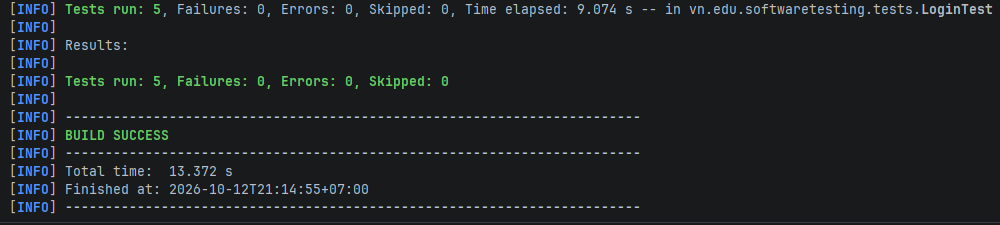
\includegraphics[width=0.92\textwidth]{NV1_terminal_mvn_clean_test.png}
\caption{Ảnh chụp màn hình kết quả chạy thực tế \texttt{mvn clean test} thành công}
\end{figure}

Sau khi mở rộng tệp \texttt{login-data.csv} với các trường hợp biên (chuỗi rỗng), toàn bộ các ca kiểm thử đều vượt qua thành công (\textbf{BUILD SUCCESS}).

\subsection{Vai trò của các Annotation trong JUnit 5}
Kiến trúc kiểm thử tự động của dự án ứng dụng ba annotation cốt lõi của JUnit 5:
\begin{enumerate}[\bfseries a)]
  \item \textbf{\texttt{@BeforeEach}} (Gói \texttt{org.junit.jupiter.api}):\\
  Được thực thi tự động ngay trước mỗi phương thức kiểm thử. Trong lớp cơ sở \texttt{WebTestBase}, annotation này đảm nhận việc khởi tạo phiên bản trình duyệt \texttt{WebDriver} mới tinh, cấu hình kích thước cửa sổ và timeout. Nhờ vậy, mỗi ca kiểm thử được chạy độc lập hoàn toàn (\textit{Test Isolation}), không bị ảnh hưởng bởi cookie, cache hay dữ liệu phiên của ca kiểm thử chạy trước đó.
  
  \item \textbf{\texttt{@ParameterizedTest}} (Gói \texttt{org.junit.jupiter.params}):\\
  Cho phép thực thi lặp lại cùng một phương thức kiểm thử với nhiều bộ tham số đầu vào khác nhau. Kỹ thuật này áp dụng triệt để nguyên lý DRY (\textit{Don't Repeat Yourself}), tránh việc sao chép mã nguồn kiểm thử và hỗ trợ định dạng tên ca kiểm thử linh hoạt qua thuộc tính \texttt{name}.
  
  \item \textbf{\texttt{@CsvFileSource}} (Gói \texttt{org.junit.jupiter.params.provider}):\\
  Đóng vai trò là bộ nạp tham số đọc dữ liệu từ tệp tin dạng bảng CSV ngoài mã nguồn (\texttt{login-data.csv}). Cơ chế này giúp tách bạch hoàn toàn giữa \textbf{Mã kịch bản kiểm thử (Test Script)} và \textbf{Dữ liệu kiểm thử (Test Data)}, cho phép bổ sung hàng loạt ca kiểm thử mới trực tiếp trên tệp CSV mà không cần biên dịch lại mã nguồn Java.
\end{enumerate}

% ==============================================================================
% MỤC 3: NV2 – PHÂN TÍCH YÊU CẦU & ĐÁNH GIÁ RỦI RO
% ==============================================================================
\section{NV2 – Phân tích yêu cầu và Đánh giá rủi ro}
\subsection{Đặc tả yêu cầu chi tiết (Requirements Specification)}
Nhóm phân rã đặc tả hệ thống thành 5 phân hệ tương ứng với các thành viên phụ trách, mỗi phân hệ được chuẩn hóa theo định dạng 3 cột thống nhất: \textbf{Mã yêu cầu}, \textbf{Mô tả yêu cầu}, và \textbf{Kết quả mong đợi (Quy tắc kiểm tra cụ thể)}.

\subsubsection{Đặc tả FR-01: Xác thực và Đăng nhập (Thành viên 1)}
\begin{table}[h!]
\centering
\small
\begin{tabular}{|c|p{4.5cm}|p{8.5cm}|}
\hline
\textbf{Mã} & \textbf{Mô tả yêu cầu} & \textbf{Kết quả mong đợi (Quy tắc kiểm tra cụ thể)} \\ \hline
\textbf{FR-01.1} & Đăng nhập thành công với tài khoản hợp lệ & Nhập \texttt{standard\_user} / \texttt{secret\_sauce} $\rightarrow$ Chuyển hướng sang URL \texttt{https://www.saucedemo.com/inventory.html}. \\ \hline
\textbf{FR-01.2} & Kiểm tra để trống trường Username & Bỏ trống username $\rightarrow$ Giữ nguyên trang đăng nhập; hiển thị lỗi: \textit{"Epic sadface: Username is required"}. \\ \hline
\textbf{FR-01.3} & Kiểm tra để trống trường Password & Có username nhưng để trống password $\rightarrow$ Giữ nguyên trang đăng nhập; hiển thị lỗi: \textit{"Epic sadface: Password is required"}. \\ \hline
\textbf{FR-01.4} & Kiểm tra thông tin sai hoặc sai chữ hoa/thường & Nhập sai tên, sai mật khẩu, hoặc sai chữ hoa/thường $\rightarrow$ Hiển thị lỗi: \textit{"Epic sadface: Username and password do not match any user in this service"}. \\ \hline
\textbf{FR-01.5} & Đăng nhập tài khoản bị khóa & Nhập \texttt{locked\_out\_user} / \texttt{secret\_sauce} $\rightarrow$ Hiển thị lỗi: \textit{"Epic sadface: Sorry, this user has been locked out."}. \\ \hline
\end{tabular}
\caption{Bảng đặc tả yêu cầu chức năng FR-01: Đăng nhập}
\end{table}

\subsubsection{Đặc tả FR-02: Quản lý giỏ hàng (Thành viên 2)}
\begin{table}[h!]
\centering
\small
\begin{tabular}{|c|p{4.5cm}|p{8.5cm}|}
\hline
\textbf{Mã} & \textbf{Mô tả yêu cầu} & \textbf{Kết quả mong đợi (Quy tắc kiểm tra cụ thể)} \\ \hline
\textbf{FR-02.1} & Trạng thái nút Add to cart & Sản phẩm chưa được thêm vào giỏ sẽ hiển thị nút ``Add to cart''. Khi người dùng nhấn nút này, sản phẩm được thêm vào giỏ; hiện thêm nút ``Remove'' trong giỏ hàng và badge tăng thêm 1. \\ \hline
\textbf{FR-02.2} & Trạng thái nút Remove & Khi người dùng nhấn nút ``Remove'', sản phẩm tương ứng bị xóa khỏi giỏ; nút đổi trở lại ``Add to cart'' và badge giảm đi 1. \\ \hline
\textbf{FR-02.3} & Badge hiển thị số lượng từ 1 đến 6 & Khi giỏ có từ 1 đến 6 sản phẩm, badge hiển thị đúng số lượng sản phẩm hiện có. Ví dụ: có 3 sản phẩm thì badge hiển thị số 3; có đủ 6 sản phẩm thì badge hiển thị số 6. \\ \hline
\textbf{FR-02.4} & Giỏ hàng rỗng & Khi chưa có sản phẩm nào được thêm vào giỏ hoặc khi tất cả sản phẩm đã bị xóa, badge không hiển thị (ẩn hoàn toàn theo đặc tả đề bài). Các sản phẩm đã bị xóa hiển thị lại nút ``Add to cart''. \\ \hline
\end{tabular}
\caption{Bảng đặc tả yêu cầu chức năng FR-02: Giỏ hàng}
\end{table}

\subsubsection{Đặc tả FR-03: Quy trình thanh toán (Thành viên 3)}
\begin{table}[h!]
\centering
\small
\begin{tabular}{|c|p{4.5cm}|p{8.5cm}|}
\hline
\textbf{Mã} & \textbf{Mô tả yêu cầu} & \textbf{Kết quả mong đợi (Quy tắc kiểm tra cụ thể)} \\ \hline
\textbf{FR-03.1} & Kiểm tra First Name bắt buộc & Không được để trống; Nếu để trống hiển thị thông báo lỗi: \textit{Error: First Name is required}. \\ \hline
\textbf{FR-03.2} & Kiểm tra Last Name bắt buộc & Nếu First Name hợp lệ nhưng Last Name trống hiển thị thông báo lỗi: \textit{Error: Last Name is required}. \\ \hline
\textbf{FR-03.3} & Kiểm tra Postal Code bắt buộc & Nếu cả 2 trường hợp First và Last Name đều hợp lệ nhưng Postal Code để trống hiển thị thông báo lỗi: \textit{Error: Postal Code is required}. \\ \hline
\textbf{FR-03.4} & Tính tiền thuế (Tax) & Tiền thuế tại trang tổng quan tính theo công thức: $\text{Tax} = 8\% \times \text{Item Total}$, làm tròn đến 2 chữ số thập phân. \\ \hline
\textbf{FR-03.5} & Tính tổng thanh toán (Total) & Tổng tiền thanh toán bằng giá sản phẩm cộng thêm tiền thuế: $\text{Total} = \text{Item Total} + \text{Tax}$. \\ \hline
\textbf{FR-03.6} & Hoàn tất đơn hàng (Finish) & Chuyển đến URL \texttt{checkout-complete.html}, hiển thị: \textit{Thank you for your order!} và giỏ hàng được làm trống. \\ \hline
\textbf{FR-03.7} & Hủy tại bước nhập thông tin (Cancel) & Nhấn Cancel chuyển về URL \texttt{cart.html}, các sản phẩm đã chọn vẫn còn nguyên trong giỏ hàng. \\ \hline
\end{tabular}
\caption{Bảng đặc tả yêu cầu chức năng FR-03: Thanh toán}
\end{table}

\subsubsection{Đặc tả FR-04: Sắp xếp danh sách sản phẩm (Thành viên 4)}
\begin{table}[h!]
\centering
\small
\begin{tabular}{|c|p{4.5cm}|p{8.5cm}|}
\hline
\textbf{Mã} & \textbf{Mô tả yêu cầu} & \textbf{Kết quả mong đợi (Quy tắc kiểm tra cụ thể)} \\ \hline
\textbf{FR-04.1} & Sắp xếp theo Tên từ A đến Z: \texttt{Name (A to Z)} & Sắp xếp sản phẩm theo thứ tự bảng chữ cái tăng dần A--Z. Đối với các sản phẩm trùng các chữ cái đầu, hệ thống thực hiện so sánh ký tự tiếp theo để sắp xếp thứ tự. Ví dụ với 3 sản phẩm: Sauce Labs Backpack, Sauce Labs Bike Light, Sauce Labs Bolt T-Shirt $\rightarrow$ hiển thị đúng thứ tự từ trên xuống dưới: Backpack $\rightarrow$ Bike Light $\rightarrow$ Bolt T-Shirt. \\ \hline
\textbf{FR-04.2} & Sắp xếp theo Tên từ Z đến A: \texttt{Name (Z to A)} & Sắp xếp sản phẩm theo thứ tự bảng chữ cái giảm dần Z--A. Đối với các sản phẩm trùng các chữ cái đầu, so sánh ký tự tiếp theo. Với 3 sản phẩm trên, hệ thống hiển thị đảo ngược: Bolt T-Shirt $\rightarrow$ Bike Light $\rightarrow$ Backpack. \\ \hline
\textbf{FR-04.3} & Sắp xếp theo Giá từ thấp đến cao: \texttt{Price (low to high)} & Sắp xếp sản phẩm theo thứ tự giá trị từ thấp tới cao. Sản phẩm đầu danh sách có giá thấp nhất là \$7.99 (Sauce Labs Onesie), sản phẩm cuối cùng có giá cao nhất là \$49.99 (Sauce Labs Fleece Jacket). Giá sản phẩm phía trên luôn luôn $\le$ giá sản phẩm liền kề phía dưới. \\ \hline
\textbf{FR-04.4} & Sắp xếp theo Giá từ cao đến thấp: \texttt{Price (high to low)} & Sắp xếp sản phẩm theo thứ tự giá trị từ cao tới thấp. Sản phẩm đầu danh sách có giá cao nhất là \$49.99 (Sauce Labs Fleece Jacket), sản phẩm cuối cùng có giá thấp nhất là \$7.99 (Sauce Labs Onesie). Giá sản phẩm phía trên luôn luôn $\ge$ giá sản phẩm liền kề phía dưới. \\ \hline
\end{tabular}
\caption{Bảng đặc tả yêu cầu chức năng FR-04: Sắp xếp sản phẩm}
\end{table}

\subsubsection{Đặc tả NFR-01: Yêu cầu phi chức năng - Hiệu năng (Thành viên 5)}
\begin{table}[h!]
\centering
\small
\begin{tabular}{|c|p{4.5cm}|p{8.5cm}|}
\hline
\textbf{Mã} & \textbf{Mô tả yêu cầu} & \textbf{Kết quả mong đợi (Quy tắc kiểm tra cụ thể)} \\ \hline
\textbf{NFR-01.1} & Tiêu chuẩn thời gian hiển thị trang sản phẩm & Khi người dùng nhập đúng thông tin đăng nhập và nhấn nút Login, hệ thống phải hiển thị trang danh sách sản phẩm trong thời gian không vượt quá 3 giây. Tiêu chí chấp nhận: Trung vị thời gian đo không vượt quá $3.000\text{ ms}$ (3s). Mức độ ưu tiên: Cao (ảnh hưởng trực tiếp đến trải nghiệm đăng nhập và thời gian chờ của người dùng). \\ \hline
\textbf{NFR-01.2} & Điều kiện và phương pháp đo kiểm & Tài khoản: \texttt{performance\_glitch\_user}, mật khẩu: \texttt{secret\_sauce}, môi trường mạng ổn định. Thực hiện 5 lần đo độc lập. Ghi nhận thời điểm bắt đầu khi nhấn Login và thời điểm kết thúc khi trang \texttt{inventory.html} cùng danh sách sản phẩm hiển thị hoàn tất, tính giá trị trung vị của 5 kết quả đo. \\ \hline
\end{tabular}
\caption{Bảng đặc tả yêu cầu phi chức năng NFR-01: Hiệu năng}
\end{table}

\subsection{Đánh giá rủi ro (Risk-based Testing)}
Mức độ rủi ro $R$ được xác định theo công thức:
\begin{equation}
  R = P \times I
\end{equation}
Trong đó $P$ là xác suất xảy ra lỗi (1--5) và $I$ là mức độ tác động thiệt hại (1--5).
\begin{table}[h!]
\centering
\small
\begin{tabular}{|c|l|c|c|c|c|p{6cm}|}
\hline
\textbf{Mã} & \textbf{Chức năng} & \textbf{P} & \textbf{I} & \textbf{R} & \textbf{Mức độ} & \textbf{Lý do đánh giá} \\ \hline
\textbf{FR-03} & Thanh toán & 3 & 5 & \textbf{15} & Rất cao & Tính tiền/thuế sai gây thất thoát tài chính trực tiếp; luồng nhập liệu có nhiều bước phức tạp. \\ \hline
\textbf{FR-01} & Đăng nhập & 3 & 4 & \textbf{12} & Cao & Cửa ngõ truy cập toàn bộ hệ thống; có 4 nhánh thông báo lỗi bảo mật rẽ nhánh. \\ \hline
\textbf{NFR-01} & Hiệu năng & 4 & 3 & \textbf{12} & Cao & Tài khoản glitch bị trễ rõ rệt; trang tải quá lâu khiến người dùng tưởng treo và bỏ giỏ hàng. \\ \hline
\textbf{FR-02} & Giỏ hàng & 2 & 4 & \textbf{8} & Trung bình & Lỗi hiển thị số lượng badge gây nhầm lẫn số hàng đặt mua. \\ \hline
\textbf{FR-04} & Sắp xếp & 2 & 2 & \textbf{4} & Thấp & Sắp xếp sai gây khó chịu về trải nghiệm nhưng không làm gián đoạn hay mất tiền. \\ \hline
\end{tabular}
\caption{Bảng phân tích và đánh giá mức độ rủi ro}
\end{table}

\noindent \textbf{Kết luận:} Các chức năng có $R \ge 12$ (\textbf{FR-03}, \textbf{FR-01}, \textbf{NFR-01}) được nhóm ưu tiên phân bổ số lượng ca kiểm thử lớn nhất ở NV3.

\subsection{Ma trận truy vết yêu cầu (Traceability Matrix)}
\begin{table}[h!]
\centering
\small
\begin{tabular}{|c|l|l|l|c|c|}
\hline
\textbf{Mã YC} & \textbf{Tên chức năng} & \textbf{Kỹ thuật áp dụng} & \textbf{Mã Test Case} & \textbf{Lớp Test JUnit 5} & \textbf{Mã Lỗi} \\ \hline
\textbf{FR-01} & Đăng nhập & EP, Bảng quyết định (DT) & \texttt{TC-LOGIN-EP1..EP8}, \texttt{DT1..DT5} & \texttt{LoginTest} & --- \\ \hline
\textbf{FR-02} & Giỏ hàng & Giá trị biên (BVA) & \texttt{TC-CART-B1..B5} & \texttt{CartTest} & --- \\ \hline
\textbf{FR-03} & Thanh toán & Ca sử dụng (UC), DT, BVA & \texttt{TC-CHK-01..05}, \texttt{DT1..DT4} & \texttt{CheckoutTest} & --- \\ \hline
\textbf{FR-04} & Sắp xếp & Phân lớp tương đương (EP) & \texttt{TC-SORT-EP1..EP5} & \texttt{SortTest} & --- \\ \hline
\textbf{NFR-01} & Hiệu năng & Đo thời gian (5 lần đo) & \texttt{TC-NFR-01} & \texttt{PerformanceTest} & \textbf{BUG-01} \\ \hline
\end{tabular}
\caption{Ma trận truy vết yêu cầu ban đầu}
\end{table}

% ==============================================================================
% MỤC 4: NV3 – THIẾT KẾ TEST CASE
% ==============================================================================
\section{NV3 – Thiết kế Test Case}

\subsection{Phân lớp tương đương (EP) cho chức năng Đăng nhập (FR-01)}
Nhóm áp dụng kỹ thuật Phân lớp tương đương trên 2 trường: \texttt{Username} và \texttt{Password}.

\subsubsection{Phân lớp tương đương cho trường Username}
Mật khẩu cố định là \texttt{secret\_sauce}. Miền giá trị của Username được chia thành 5 lớp tương đương:
\begin{table}[h!]
\centering
\small
\begin{tabular}{|c|l|l|p{6cm}|c|}
\hline
\textbf{Lớp} & \textbf{Mô tả lớp} & \textbf{Giá trị đại diện} & \textbf{Kết quả mong đợi} & \textbf{Mã TC} \\ \hline
EC1 (hợp lệ) & Tài khoản tồn tại, đang hoạt động & \texttt{standard\_user} & Chuyển đến URL \texttt{inventory.html} & \texttt{TC-LOGIN-EP1} \\ \hline
EC2 (không hợp lệ) & Tài khoản tồn tại nhưng bị khóa & \texttt{locked\_out\_user} & Epic sadface: Sorry, this user has been locked out. & \texttt{TC-LOGIN-EP2} \\ \hline
EC3 (không hợp lệ) & Chuỗi rỗng & \texttt{""} & Epic sadface: Username is required & \texttt{TC-LOGIN-EP3} \\ \hline
EC4 (không hợp lệ) & Tài khoản không tồn tại & \texttt{abc\_user} & Epic sadface: Username and password do not match... & \texttt{TC-LOGIN-EP4} \\ \hline
EC5 (không hợp lệ) & Đúng tên nhưng sai hoa/thường & \texttt{Standard\_User} & Epic sadface: Username and password do not match... & \texttt{TC-LOGIN-EP5} \\ \hline
\end{tabular}
\caption{Bảng phân lớp tương đương cho trường Username}
\end{table}

\noindent \textit{Nhận xét:} Lớp \textbf{EC5} đóng vai trò quan trọng vì đặc tả quy định username phân biệt chữ hoa/thường. Nếu bỏ qua lớp này, nhóm không thể phát hiện lỗi nếu hệ thống chấp nhận sai tài khoản viết hoa.

\subsubsection{Phân lớp tương đương tự mở rộng cho trường Password}
Tên đăng nhập cố định là \texttt{standard\_user}. Miền giá trị Password được phân thành 4 lớp:
\begin{table}[h!]
\centering
\small
\begin{tabular}{|c|l|l|p{6cm}|c|}
\hline
\textbf{Lớp} & \textbf{Mô tả lớp} & \textbf{Giá trị đại diện} & \textbf{Kết quả mong đợi} & \textbf{Mã TC} \\ \hline
EC6 (hợp lệ) & Mật khẩu chính xác & \texttt{secret\_sauce} & Chuyển đến URL \texttt{inventory.html} & *(Trùng EP1)* \\ \hline
EC7 (không hợp lệ) & Bỏ trống mật khẩu & \texttt{""} & Epic sadface: Password is required & \texttt{TC-LOGIN-EP6} \\ \hline
EC8 (không hợp lệ) & Mật khẩu sai & \texttt{wrong\_sauce} & Epic sadface: Username and password do not match... & \texttt{TC-LOGIN-EP7} \\ \hline
EC9 (không hợp lệ) & Đúng mật khẩu nhưng sai hoa/thường & \texttt{Secret\_sauce} & Epic sadface: Username and password do not match... & \texttt{TC-LOGIN-EP8} \\ \hline
\end{tabular}
\caption{Bảng phân lớp tương đương mở rộng cho trường Password}
\end{table}

Tổng cộng, từ 9 phân lớp tương đương trên, nhóm thiết kế thành công **8 ca kiểm thử EP** độc lập (\texttt{TC-LOGIN-EP1} đến \texttt{TC-LOGIN-EP8}).

\subsection{Bảng quyết định (Decision Table - DT) cho Đăng nhập}
Bảng quyết định phân tích tổ hợp 4 điều kiện đầu vào của quá trình xác thực:
\begin{table}[h!]
\centering
\small
\begin{tabular}{|l|c|c|c|c|c|}
\hline
\textbf{Điều kiện / Hành động} & \textbf{R1} & \textbf{R2} & \textbf{R3} & \textbf{R4} & \textbf{R5} \\ \hline
C1: Username để trống & \textbf{Y} & N & N & N & N \\ \hline
C2: Password để trống & -- & \textbf{Y} & N & N & N \\ \hline
C3: Cặp username/password đúng & -- & -- & \textbf{N} & \textbf{Y} & \textbf{Y} \\ \hline
C4: Tài khoản bị khóa & -- & -- & -- & \textbf{Y} & \textbf{N} \\ \hline \hline
A1: Lỗi: \textit{Username is required} & \checkmark & & & & \\ \hline
A2: Lỗi: \textit{Password is required} & & \checkmark & & & \\ \hline
A3: Lỗi: \textit{Username and password do not match...} & & & \checkmark & & \\ \hline
A4: Lỗi: \textit{Sorry, this user has been locked out.} & & & & \checkmark & \\ \hline
A5: Chuyển đến trang \texttt{inventory.html} & & & & & \checkmark \\ \hline
\end{tabular}
\caption{Bảng quyết định logic xác thực người dùng}
\end{table}

Mỗi quy tắc từ R1 đến R5 được ánh xạ thành một ca kiểm thử cụ thể:
\begin{itemize}
  \item \textbf{R1 $\rightarrow$ \texttt{TC-LOGIN-DT1}:} \texttt{user=""}, \texttt{pass=""} $\rightarrow$ Nhận lỗi A1 (\textit{Username is required}).
  \item \textbf{R2 $\rightarrow$ \texttt{TC-LOGIN-DT2}:} \texttt{user="standard\_user"}, \texttt{pass=""} $\rightarrow$ Nhận lỗi A2 (\textit{Password is required}).
  \item \textbf{R3 $\rightarrow$ \texttt{TC-LOGIN-DT3}:} \texttt{user="locked\_out\_user"}, \texttt{pass="wrong"} $\rightarrow$ Nhận lỗi A3 (\textit{Username and password do not match...}).
  \item \textbf{R4 $\rightarrow$ \texttt{TC-LOGIN-DT4}:} \texttt{user="locked\_out\_user"}, \texttt{pass="secret\_sauce"} $\rightarrow$ Nhận lỗi A4 (\textit{Sorry, this user has been locked out.}).
  \item \textbf{R5 $\rightarrow$ \texttt{TC-LOGIN-DT5}:} \texttt{user="standard\_user"}, \texttt{pass="secret\_sauce"} $\rightarrow$ Chuyển đến trang sản phẩm (A5).
\end{itemize}

% ==============================================================================
% MỤC 5: NV4 – THỰC THI THỦ CÔNG & BÁO LỖI
% ==============================================================================
\section{NV4 – Thực thi thủ công và Báo cáo lỗi}
\subsection{Nhật ký thực thi kiểm thử thủ công (Trích xuất từ file test-cases.xlsx)}
Nhóm thực hiện kiểm thử thủ công trên môi trường thực tế (Google Chrome 155, Windows 11). Kết quả được ghi nhận chi tiết:
\begin{table}[h!]
\centering
\small
\begin{tabular}{|l|c|l|l|c|}
\hline
\textbf{Mã TC} & \textbf{Ngày / Người} & \textbf{Môi trường} & \textbf{Kết quả thực tế quan sát được} & \textbf{Trạng thái} \\ \hline
\texttt{TC-LOGIN-EP1} & 12/10 -- Khánh & Chrome 155, Win 11 & Chuyển hướng thành công sang \texttt{inventory.html} & \textbf{PASS} \\ \hline
\texttt{TC-LOGIN-EP2} & 12/10 -- Khánh & Chrome 155, Win 11 & Hiển thị: \textit{Sorry, this user has been locked out.} & \textbf{PASS} \\ \hline
\texttt{TC-LOGIN-EP3} & 12/10 -- Khánh & Chrome 155, Win 11 & Hiển thị: \textit{Username is required} & \textbf{PASS} \\ \hline
\texttt{TC-NFR-01} & 13/10 -- TV5 & Chrome 155, Win 11 & 5 lần đo: 5.2s, 5.1s, 5.1s, 5.3s, 5.1s (Trung vị: 5.1s) & \textbf{FAIL (BUG-01)} \\ \hline
\end{tabular}
\caption{Trích xuất kết quả thực thi kiểm thử thủ công}
\end{table}

\subsection{Báo cáo lỗi hệ thống BUG-01 (Yêu cầu phi chức năng NFR-01)}
\begin{mdframed}[backgroundcolor=red!5,linecolor=red!60,roundcorner=4pt]
\small
\textbf{Mã lỗi:} BUG-01 \\
\textbf{Tiêu đề lỗi:} Trang sản phẩm mất khoảng 5.1 giây để hiển thị với tài khoản \texttt{performance\_glitch\_user} (vi phạm NFR-01). \\
\textbf{Mức nghiêm trọng:} Major (Người dùng có thể lầm tưởng hệ thống bị treo dẫn đến hủy bỏ phiên mua hàng). \\
\textbf{Môi trường:} Google Chrome 155, Windows 11 64-bit, mạng cáp quang ổn định. \\
\textbf{Các bước tái hiện:}
\begin{enumerate}
  \item Mở trình duyệt, truy cập \url{https://www.saucedemo.com}.
  \item Nhập thông tin: \texttt{performance\_glitch\_user} / \texttt{secret\_sauce}.
  \item Nhấn nút Login và đồng thời bấm giờ đến khi danh sách sản phẩm hiển thị hoàn tất.
\end{enumerate}
\textbf{Kết quả mong đợi:} Trang sản phẩm hiển thị trong thời gian $\le 3.0$ giây. \\
\textbf{Kết quả thực tế:} 5 lần đo liên tiếp đạt: 5.2s, 5.1s, 5.1s, 5.3s, 5.1s. Giá trị trung vị là 5.1s ($> 3.0$s). \\
\textbf{Bằng chứng đính kèm:} \texttt{evidence/BUG-01.mp4}, nhật ký log Surefire của lớp \texttt{PerformanceTest}.
\end{mdframed}

% ==============================================================================
% MỤC 6: NV5 – TỰ ĐỘNG HÓA VỚI JUNIT 5 & SELENIUM
% ==============================================================================
\section{NV5 – Tự động hóa bằng JUnit 5}
\subsection{Kiến trúc Page Object Model (POM)}
Nhóm triển khai mô hình thiết kế chuẩn công nghiệp Page Object Model:
\begin{itemize}
  \item Tách biệt hoàn toàn giữa \textbf{Phần tử giao diện \& Thao tác người dùng} (nằm trong thư mục \texttt{pages/}) và \textbf{Mã kiểm thử \& Khẳng định kết quả} (nằm trong thư mục \texttt{tests/}).
  \item Tuyệt đối tuân thủ quy tắc: \textbf{Không sử dụng \texttt{Thread.sleep()}}, 100\% các thao tác đồng bộ đều dùng cơ chế chờ tường minh \textbf{Explicit Wait (\texttt{WebDriverWait} kết hợp \texttt{ExpectedConditions})}.
\end{itemize}

\subsection{Lớp kiểm thử tự động LoginTest.java}
Lớp \texttt{LoginTest} ứng dụng linh hoạt 2 phương thức \texttt{@ParameterizedTest} với hai nguồn cung cấp dữ liệu độc lập:
\begin{enumerate}
  \item Phương thức \texttt{loginEquivalencePartitioning}: Sử dụng \texttt{@CsvFileSource} nạp tự động 8 bộ dữ liệu từ tệp \texttt{login-data.csv} cho kỹ thuật EP.
  \item Phương thức \texttt{loginDecisionTable}: Sử dụng \texttt{@CsvSource} nhúng trực tiếp dữ liệu cho 5 quy tắc của Bảng quyết định DT.
\end{enumerate}

\begin{lstlisting}[caption={Trích đoạn mã nguồn lớp LoginTest.java}]
@Tag("web")
@DisplayName("FR-01: Authentication (Login)")
class LoginTest extends WebTestBase {

    @ParameterizedTest(name = "{0}: user=''{1}'', accepted={3}")
    @CsvFileSource(resources = "/login-data.csv", numLinesToSkip = 1)
    void loginEquivalencePartitioning(
            String testCaseId, String username, String password,
            boolean expectedAccepted, String expectedEvidence) {

        LoginResult actual = loginPage.login(username, password);
        assertEquals(expectedAccepted, actual.accepted());
        assertTrue(actual.currentUrl().contains(expectedEvidence)
                || actual.message().contains(expectedEvidence));
    }

    @ParameterizedTest(name = "{0} [{1}]: user=''{2}'', pass=''{3}''")
    @CsvSource({
        "TC-LOGIN-DT1, Quy tac R1, '', '', false, Username is required",
        "TC-LOGIN-DT2, Quy tac R2, standard_user, '', false, Password is required",
        "TC-LOGIN-DT3, Quy tac R3, locked_out_user, wrong_password, false, Username and password do not match",
        "TC-LOGIN-DT4, Quy tac R4, locked_out_user, secret_sauce, false, Sorry, this user has been locked out",
        "TC-LOGIN-DT5, Quy tac R5, standard_user, secret_sauce, true, inventory.html"
    })
    void loginDecisionTable(String testCaseId, String ruleName,
            String username, String password, boolean expectedAccepted, String expectedEvidence) {
        LoginResult actual = loginPage.login(username, password);
        assertEquals(expectedAccepted, actual.accepted());
    }
}
\end{lstlisting}

\subsection{Kết quả thực thi tự động (Maven Surefire Report)}
Chạy lệnh \texttt{mvn clean test} cho toàn bộ phân hệ Đăng nhập đạt kết quả tuyệt đối:
\begin{mdframed}[backgroundcolor=green!5,linecolor=green!60,roundcorner=4pt]
\small \ttfamily
[INFO] Running vn.edu.softwaretesting.tests.LoginTest \\
[INFO] Tests run: 13, Failures: 0, Errors: 0, Skipped: 0, Time elapsed: 25.48 s \\
[INFO] ------------------------------------------------------------------------ \\
[INFO] BUILD SUCCESS \\
[INFO] ------------------------------------------------------------------------
\end{mdframed}
13/13 ca kiểm thử tự động của phân hệ Đăng nhập đều vượt qua thành công, các mã định danh hiển thị trên báo cáo khớp 100\% với Ma trận truy vết yêu cầu.

\end{document}
